\chapter{Notes}
\label{ch:notes}

\todo[inline]{Remove Notes before releasing.}

% ------------------------------------------------------------------------------
\section{Weighted Sum MKN Algorithm from Code}

\begin{algorithm}
  \caption{Weighted Sum MKN algo from Code (likely optimizable)}
  \begin{algorithmic}[1]
    \Require $h$
      \Comment{History for which to determinate interpolation weights}
    \Ensure $\SumWeight_i^h$
      \Comment{Array of interpolation weights}

    \LineComment{Find first seen history $\SeenHistory$}
    \State $\SeenHistory \gets h$
    \While{$\Count(\SeenHistory \Skp) = 0$}
      \State $\SeenHistory \gets \SeenHistory\text{.backoff()}$
             \todo[inline]{Better notation for backoff}
    \EndWhile
    \State $N = \NGramLength{\SeenHistory} + 1$
    \State $\SumWeight^h \gets$ new array of size $N$
    %\State
    \State $nominator \gets 1$
    \State $denominator \gets \Count(\SeenHistory \Skp)$
    \State $\SumWeight_1^h \gets \frac{1}{denominator}$
    %\State
    \State $\DerivedHistory \gets \SeenHistory$
    \For{$i \gets 2, N$}
      \State $nominator \gets \gamma(\DerivedHistory) \frac{nominator}{denominator}$
      \State $\DerivedHistory \gets \DerivedHistory\text{.backoff()}$
      \State $denominator \gets \ContCountIp(\WSkp \DerivedHistory \WSkp)$
      \State $\SumWeight_i^h \gets \frac{nominator}{denominator}$
    \EndFor
  \end{algorithmic}
\end{algorithm}

% ------------------------------------------------------------------------------
\clearpage
\section{Alternative Binomial Diamond of order 3}

\begin{figure}[H]
  \centering
  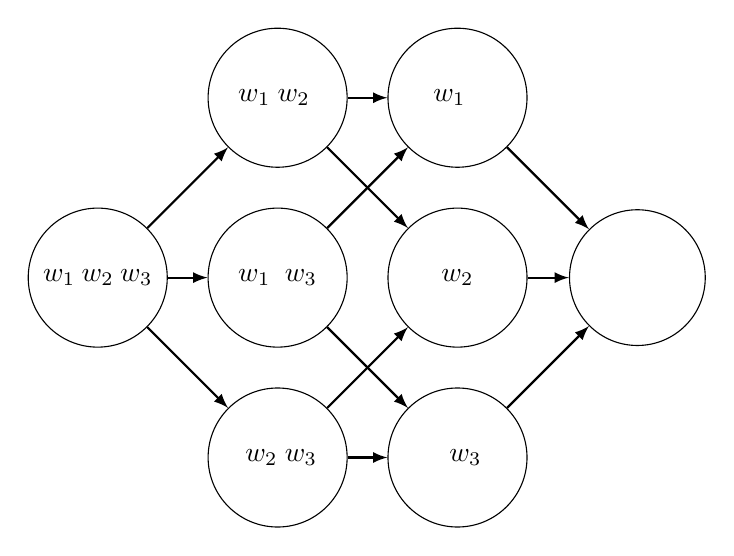
\begin{tikzpicture}[
    node distance = 6.5em,
    seq/.style = {draw, circle, align=center, text centered, text width=4.2em},
  ]
    \node [seq] (000)                {$w_1 \: w_2 \: w_3$};

    \node [seq] (010) [right of=000] {$w_1 \: \Skp \: w_3$};
    \node [seq] (001) [above of=010] {$w_1 \: w_2 \: \Skp$};
    \node [seq] (100) [below of=010] {$\Skp \: w_2 \: w_3$};

    \node [seq] (101) [right of=010] {$\Skp \: w_2 \: \Skp$};
    \node [seq] (011) [above of=101] {$w_1 \: \Skp \: \Skp$};
    \node [seq] (110) [below of=101] {$\Skp \: \Skp \: w_3$};

    \node [seq] (111) [right of=101] {$\Skp \: \Skp \: \Skp$};

    \path[->, >=latex, thick]
      (000) edge (001)
      (000) edge (010)
      (000) edge (100)

      (001) edge (011)
      (001) edge (101)
      (010) edge (011)
      (010) edge (110)
      (100) edge (101)
      (100) edge (110)

      (011) edge (111)
      (101) edge (111)
      (110) edge (111);
  \end{tikzpicture}
\end{figure}

% ------------------------------------------------------------------------------
\begin{landscape}
  \section{Binomial Diamond of order 4}
  \begin{figure}[H]
    \centering
    \scalebox{0.7}{
      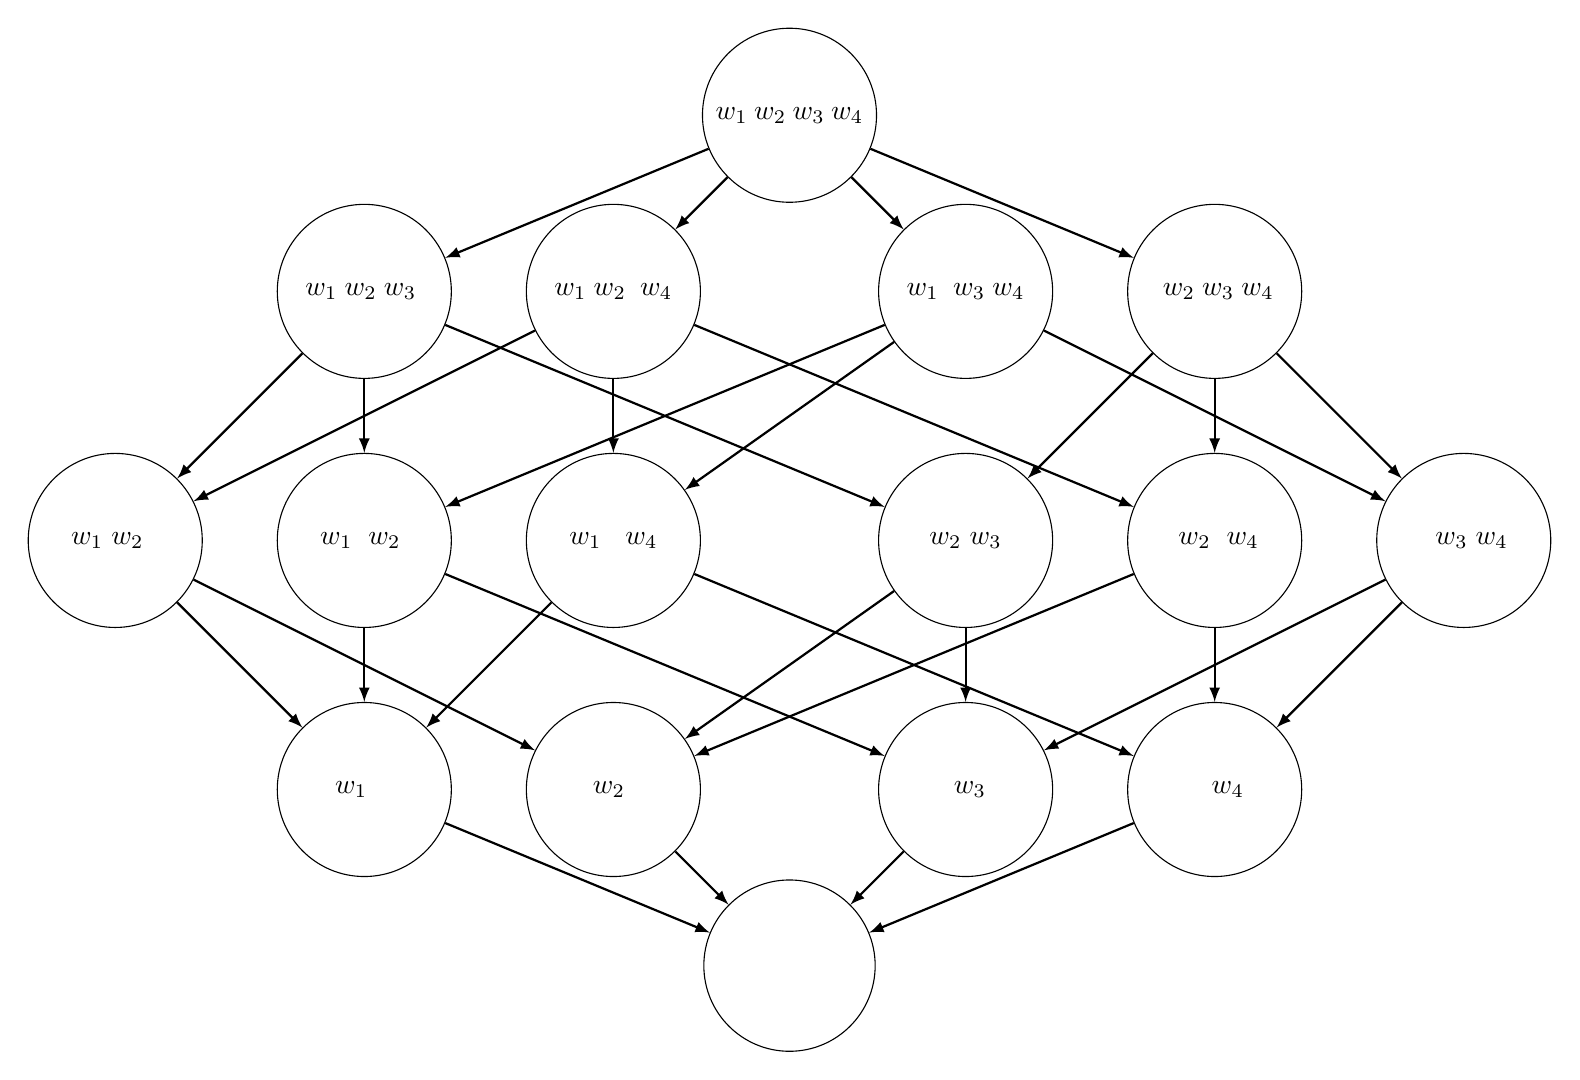
\begin{tikzpicture}[
        node distance = 9em,
        seq/.style = {draw, circle, align=center, text centered, text width=5.5em},
      ]
        \node [seq] (0000) {$w_1 \: w_2 \: w_3 \: w_4$};

        \node [seq] (0010) [below left  of=0000] {$w_1 \: w_2 \: \Skp \: w_4$};
        \node [seq] (0100) [below right of=0000] {$w_1 \: \Skp \: w_3 \: w_4$};
        \node [seq] (0001) [      left  of=0010] {$w_1 \: w_2 \: w_3 \: \Skp$};
        \node [seq] (1000) [      right of=0100] {$\Skp \: w_2 \: w_3 \: w_4$};

        \node [seq] (0101) [below       of=0001] {$w_1 \: \Skp \: w_2 \: \Skp$};
        \node [seq] (0110) [below       of=0010] {$w_1 \: \Skp \: \Skp \: w_4$};
        \node [seq] (1001) [below       of=0100] {$\Skp \: w_2 \: w_3 \: \Skp$};
        \node [seq] (1010) [below       of=1000] {$\Skp \: w_2 \: \Skp \: w_4$};
        \node [seq] (0011) [      left  of=0101] {$w_1 \: w_2 \: \Skp \: \Skp$};
        \node [seq] (1100) [      right of=1010] {$\Skp \: \Skp \: w_3 \: w_4$};

        \node [seq] (0111) [below       of=0101] {$w_1 \: \Skp \: \Skp \: \Skp$};
        \node [seq] (1011) [below       of=0110] {$\Skp \: w_2 \: \Skp \: \Skp$};
        \node [seq] (1101) [below       of=1001] {$\Skp \: \Skp \: w_3 \: \Skp$};
        \node [seq] (1110) [below       of=1010] {$\Skp \: \Skp \: \Skp \: w_4$};

        \node [seq] (1111) [below right of=1011] {$\Skp \: \Skp \: \Skp \: \Skp$};

        \path[->, >=latex, thick]
          (0000) edge (0001)
          (0000) edge (0010)
          (0000) edge (0100)
          (0000) edge (1000)

          (0001) edge (0011)
          (0001) edge (0101)
          (0001) edge (1001)
          (0010) edge (0011)
          (0010) edge (0110)
          (0010) edge (1010)
          (0100) edge (0101)
          (0100) edge (0110)
          (0100) edge (1100)
          (1000) edge (1001)
          (1000) edge (1010)
          (1000) edge (1100)

          (0011) edge (0111)
          (0011) edge (1011)
          (0101) edge (0111)
          (0101) edge (1101)
          (0110) edge (0111)
          (0110) edge (1110)
          (1001) edge (1011)
          (1001) edge (1101)
          (1010) edge (1011)
          (1010) edge (1110)
          (1100) edge (1101)
          (1100) edge (1110)

          (0111) edge (1111)
          (1011) edge (1111)
          (1101) edge (1111)
          (1110) edge (1111);
      \end{tikzpicture}
    }
  \end{figure}
\end{landscape}

% ==============================================================================
\chapter{Timeline}

\begin{itemize}
  \item Write chapters
    \begin{itemize}
      \item Introduction (1-2 days)
      \item Related Work (1 day)
      \item Review of Considered language Models (1 day)
      \item Formulating Language Models as Weighted Sums
      \item Fast Prefix Queries using Top-\emph{k} Joins
      \item Evaluation
      \item Conclusion (1-2 days)
    \end{itemize}
  \item Think of experiments and implement them (3-4 days)
  \item Find new notation for chapter weighted sums (\emph{hard to estimate})
    \begin{itemize}
      \item Needs to be able to nicely represent MKN weighted sum argument.
      \item Should be able to nicely represent GLM weighted sum argument.
      \item It would be nice if the notation makes proving MKN weighted sum.
    \end{itemize}
  \item Finishing (3-4 days)
    \begin{itemize}
      \item Fix latex
      \item Reformulate shitty sentences
      \item Check formatting
    \end{itemize}
  \item Peer review, spelling correction (1-2 weeks)
  \item Make slides, prepare presentation (1 week)
\end{itemize}

\clearpage
\hrule
\subsubsection*{Week 6.7. - 12.7.}
\begin{itemize}
  \item  6.7. Monday:
  \item  7.7. Tuesday:
  \item  8.7. Wednesday:
  \item  9.7. Thursday:
  \item 10.7. Friday:
  \item 11.7. Saturday:
  \item 12.7. Sunday;
\end{itemize}

\hrule
\subsubsection*{Week 13.7. - 19.7.}
\begin{itemize}
  \item 13.6. Monday:
  \item 14.6. Tuesday:
  \item 15.7. Wednesday:
  \item 16.7. Thursday:
  \item 17.7. Friday:
  \item 18.7. Saturday:
  \item 19.7. Sunday;
\end{itemize}

\hrule
\subsubsection*{Week 20.7. - 26.7.}
\begin{itemize}
  \item 20.6. Monday:
  \item 21.6. Tuesday:
  \item 22.7. Wednesday:
  \item 23.7. Thursday:
  \item 24.7. Friday:
  \item 25.7. Saturday:
  \item 26.7. Sunday;
\end{itemize}

\clearpage
\hrule
\subsubsection*{Week 27.7. - 2.8.}
\begin{itemize}
  \item 27.6. Monday: Need to start peer review.
  \item 28.6. Tuesday:
  \item 29.7. Wednesday:
  \item 30.7. Thursday: Need to start working on presentation.
  \item 31.7. Friday:
  \item  1.8. Saturday:
  \item  2.8. Sunday;
\end{itemize}

\hrule
\subsubsection*{Week 3.8. - 9.8.}
\begin{itemize}
  \item  3.8. Monday:
  \item  4.8. Tuesday:
  \item  5.8. Wednesday:
  \item \textbf{6.8. Thursday: Colloquium}
\end{itemize}
